
\date{\today}
\title{Traceroute Exploration}


\documentclass[12pt]{article}

\usepackage{graphicx}

\author{
  Singhal, Madhur\\
  \texttt{2015CS10235}
  \and
  Chhajwani, Anant\\
  \texttt{2015CS50281}
}

\begin{document}
\maketitle


\section{Introduction}
Traceroute is a computer network diagnostic tool for displaying the route (path) and measuring transit delays of packets across an Internet Protocol (IP) network. It works using the ICMP protocol; by varying the TTL value of the packets it sends, traceroute can find the exact path through which packets are being routed on the way to a destination.
\paragraph{}
In this assignment we use traceroute to study how networks are laid out in real life. We also study how the latency is related to the number of hops a packet must make.

\section{Number of Hops}

\begin{center}
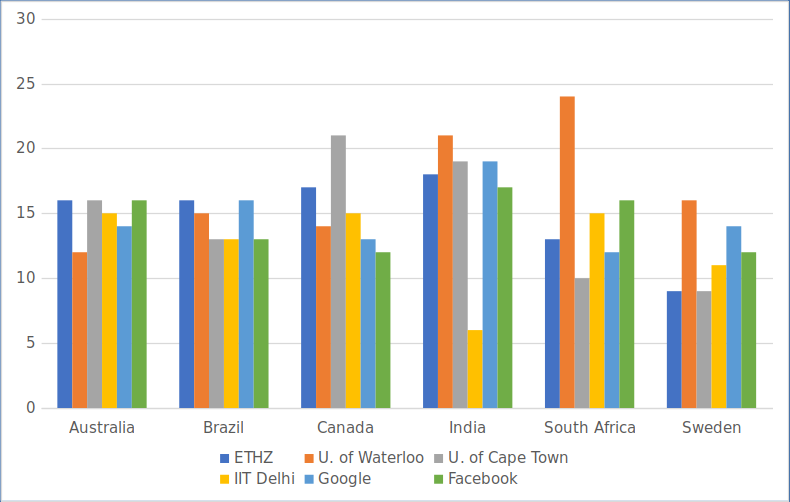
\includegraphics[scale=0.76]{ch.png}
\end{center}
The number of hops between nodes in the same continent are lower than hops between nodes
in different continents. We can understand this by abstracting internet in a form of rooted tree,
with world as root, continents as children of root, countries as children of continents and so on. Now when source and destination nodes fall in different continents, the path traced by
traceroute will reach higher up the tree towards the root and so will require higher number of
hops.
The number of hops required by Google and Facebook are different in general, since they are different
web servers located at different places.

\section{Latency}
\begin{center}
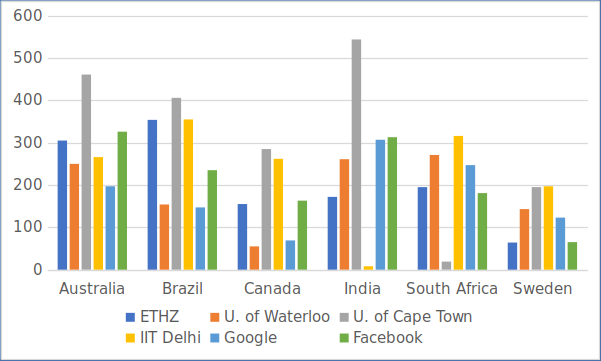
\includegraphics[scale=0.86]{lat.png}
\end{center}
We can observe from data that generally the higher is the number of hops the higher is the latency. The reason seems obvious as each hop has some contribution to the latency. A key point to note is that latency is hugely affected by inter continental hops which require underwater network cables.
\section{Peering}
No country of traceroute servers was found to have local ISPs directly peered with Google and
Facebook. Though as a separate experiment when we  rented a DigitalOcean server in NY and tracerouted to NetFlix and Google, we found it peered directly to the services, though Facebook was still not peered.

\section{Cellular Latency}

In cellular networks, the hops inside of the cellular network contribute the most to latency. Cellular networks are long range open air communications and as such the protocols designed for them have to be robust. The LTE protocol itself has very large minimum latencies for many things like handshakes  and acks. Since the IP layer etc all come above the LTE layer they have to live with the large latency of LTE and thus overall latency is also large.
 
\section{ISP connectivity}

Routes to some destinations are often reached in much fewer hops than others with the same geographical separation. Also sometimes a packet from Delhi to Beijing could be transmitted through USA even though that is geographically farther away. All this suggests that in general there is no fixed rule to predict what path a particular ISP will send a packet to. It depends to a large degree on the companies with which the ISP has contracts (or peering arrangements) about carrying packets intended towards particular destinations. 

\end{document}